\section{Inverse Texture Synthesis}
Another algorithm for summarizing images is the \textit{inverse texture synthesis} discovered by \textsc{Wei, Han, Zhou, Bao, Guo} and \textsc{Shum}.\\
It works similar to bidirectional similarity (see section 2) by comparing for completeness and coherence. Those steps only have different names (forward M-step and inverse M-step) and the algorithm does not use gradual resizing, instead the target images changes continously. \\
Inverse texture synthesis brings a user-controllable feature with it: control maps. So we will first learn about control maps and then introduce the technical details of the algorithm.

\subsection{Control maps}
As mentioned before, control maps are a big feature in inverse texture synthesis not only because they are user-controllable. Technically they are an additional layer for computation to manipulate how the final texture will look like, similar to importance weights of bidirectional similarity (section 2.3.3).\\
Figure \ref{fig:Control maps} shows an example for control maps. As you can see the control map 'controls' where the brown spots are located on the final texture. The non-black parts work like a mask to show a desired percentage of the brown spots where white means 100\% brown.\\
If we would change the white parts of the control map, the brown spots on the texture would change too.\\
User can define their own control maps to achieve different textures like painting dirt on a mesh\footnotemark  of a vase. 

\footnotetext{A \textit{mesh} is a collection of polygons in 3D computer graphics representing a 3D object.}

\begin{figure}[h]
\centering
\includegraphics[scale=0.9]{img/controlmaps}
\caption[Control maps]{On the left a texture, on the right the control map for the texture.\\ Images from \cite{its}.}
\label{fig:Control maps}
\end{figure}


\subsection{Algorithm}
The algorithm of inverse texture synthesis starts by filling the compactation with random pixels from the original image. Not only the color information from the pixel will be copied also the original location of it so it can be compared to its neighbors in the original image.\\
Like the bidirectional similarity it is a two-way comparison of patches by finding the most similar ones (section 2.1). The check for coherence is called \textit{forward M-step} and the check for completeness is called \textit{inverse M-step}.\\
The algorithm begins with the so-called \textit{z E-step} and the last step is called \textit{w E-step} where the result is manipulated by an \textit{orientation field}.

\begin{figure}[h]
\centering
\includegraphics[scale=0.75]{img/its-algo}
\caption[Inverse texture synthesis algortihm]{This figure shows different steps of the algorithm. (a) shows the z E-step and forward M-step. (b) illustrates the inverse M-step.}
\label{fig:Inverse texture synthesis algortihm}
\end{figure}

\subsubsection{z E-step}
After initializing the compactation \textit{T} with random pixels from the original image \textit{S}, the algorithm selects a pixel in \textit{T}.
Figure \ref{fig:Inverse texture synthesis algortihm} (a) shows the selected pixel $0$. Pixel $0$ has neighbors ${1,2,3,4}$ which do have a origin in the original image \textit{S}.\\
The origin was also copied when initializing the compactation with random pixels. The neighbors ${1,2,3,4}$  also have neighbors in the original image - in this case those are ${5,6,7,8}$.\\
From the neighbors ${5,6,7,8}$ the algorithm can now calculate a median color for pixel $0$.

\subsubsection{Forward M-step}
The forward M-step is similar to coherence check in bidirectional similarity. This step does not need any additional computation. For a patch $Q$ in compactation $T$ containing pixel $q$ it just looks for a best matching patch $P$ in original image $S$.\\
The example in Figure \ref{fig:Inverse texture synthesis algortihm} (a) is pixel-based, so the forward M-step could be finding the best matching pixel from ${5,6,7,8}$ to pixel $0$. This is a constant time operation and not applicable to the inverse M-step. 

\subsubsection{Inverse M-step}
The inverse M-step is similar to completeness check in bidirectional similarity. But it works different to the forward M-Step. Because of the constantly changing compactation it is not possible to save the location of the copied pixels. So comparing patches between source image $S$ and compaction $T$ is only possible by exhaustive search.\\
Figure \ref{fig:Inverse texture synthesis algortihm} (b) shows an example for the inverse M-step. If patch $B$ needs to find a similar patch in $T$ it has to do an exhaustive search. This results in a bad performance if every patch has to do an exhaustive search.\\
Inverse texture synthesis brings a faster solution: Instead of looking for a similar patch in $T$, the algorithm first looks for a similar patch in $S$. So in the example: patch $A$ matches patch $B$ and $B$ matches patch $C$ in target image $T$. So patch $A$ also matches patch $C$.\\
Every patch which matches patch $B$ also matches to patch $C$. This gives a performance boost compared to simple exhaustive search, because a search tree can be built. It is a logarithmic speed up.


\subsubsection{w E-step}
In the last step, called \textit{w E-step}, the algorithm uses an orientation field to optimize the result of compactation. It works like and additional layer of information.\\
Figure \ref{fig:Orientation field} shows some examples for orientation fields. The most important aspect to learn from here is that different orientation fields have different results in compactation.

\begin{figure}[h]
\centering
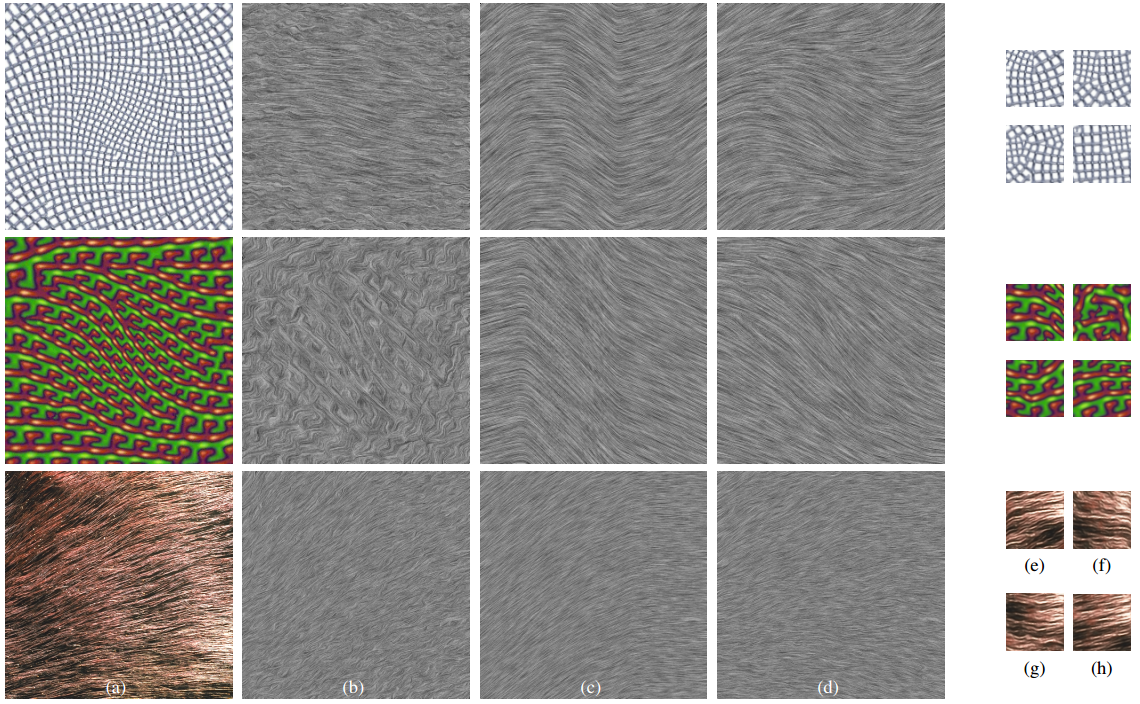
\includegraphics[scale=0.4]{img/orientationfield}
\caption[Orientation field]{This figure shows within each row different orientation fields. (a) is the orignal texture with uniform x-y-orientation. (b) shows the orientation fields from \cite{paris}. (c) shows orientation fields via manual specification followed by interpolation. And (d) is the orientation field from \cite{its} based on (c). (e), (f), (g) and (h) are the resulting images from (a), (b), (c) and (d).\\ Images from \cite{its}.}
\label{fig:Orientation field}
\end{figure}
\pagebreak

\begin{figure}[h]
\centering
\includegraphics[scale=1]{img/its-example}
\caption[Inverse texture synthesis example]{This figure shows an example usage of inverse texture synthesis. On the left is the original texture in different luminance variations and the control map. After using the algorithm, there can be found the compactation of original texture and control map. The compactations can be used for forward synthesis. There are also some calculation benchmarks between useage original texture and compactation.\\ Images by \cite{its}.}
\label{fig:Inverse texture synthesis example}
\end{figure}


\subsection{Example}
As the algorithm of bidirectional similarity the algorithm can be used in a different manner. The simplest one is to calculate a compactation for reusing it in forward synthesis.\\
Figure \ref{fig:Inverse texture synthesis example} shows such an example usage. The first step in this example is to use inverse texture synthesis to create a compaction from the original texture and the original control map.\\
The original texture has a size of 890x890 pixels in eleven different luminance variations. The original control map has the same size. The compactation size is 128x128 pixels. This compactations can now be used for texturing a mesh like the seehorse. First the (compacted) control map is used to manipulate the final look of the texture and then the orignal texture is drawn on the mesh. In this example the original texture and the compactation were used for comparison purposes. There are nearly no differences by using the compactation instead of the original texture.\\
It should also be noted that by using the compactation it is much more faster to texture the seehorse (Original texture: 14776 sec, compactation: 1719 sec).
\pagebreak

\subsection{Performance and limitations}
The performance of the inverse texture synthesis algorithm is fairly efficient and more efficient than the bidirectional similarity algorithm.\\
Figure \ref{fig:Inverse texture synthesis performance} shows an example for compactation. This compactation was achieved in 147 sec. Furthermore, the algorithm is capable of doing forward synthesis and GPU-acclelerated calculations.\\
If the control map is not reasonably enough related to the original map the compactation can not recover the original texture by forward synthesis.

\begin{figure}[h]
\centering
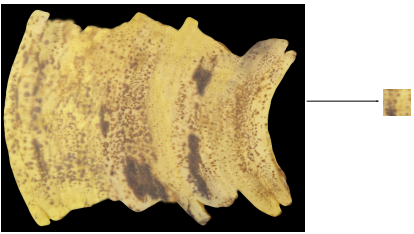
\includegraphics[scale=1]{img/its-banana}
\caption[Inverse texture synthesis performance]{An example image for performance demonstration.\\ Images by \cite{its}.}
\label{fig:Inverse texture synthesis performance}
\end{figure}